\section{Place Recognition Algorithm}
\label{sec:chap_slam_algo}

While there is quite a few articles presenting place recognition algorithms using different sensors (e.g. cameras, \gls*{gps}), the literature of such algorithms based solely on \gls*{3d} data is limited. For our place recognition analysis, we choose to evaluate on our datasets the state-of-the-art algorithm (at the time of the experiments) developed by \citet{Steder2011b}. The full details of the technique are presented in the article. However for the sake of this document, we will first describe some fundamental concepts used for place recognition in Section~\ref{ssec:chap_slam_basics} and then we will give an overview of the Steder algorithm itself in Section~\ref{ssec:chap_slam_algo}. 


\subsection{Fundamental Concepts}
\label{ssec:chap_slam_basics}

\subsubsection{Feature Keypoints and Descriptors}
\label{ssub:feature_keypoints_and_descriptors}

The first step to determine whether or not a place has been visited before by the robot, is to convert the data into a more convenient format for identification. The generally adopted representation is a vector of real numbers, called descriptor. A descriptor can be global, meaning that it tries to capture information about the whole sample, or local, meaning that it does the same but only for a specific subregion of the sample. When using local descriptors, it is first required to determine the keypoints around which the descriptors will be extracted. These keypoints can be at pre-determined and fixed locations (e.g. division in a simple grid) or selected using more refined algorithms. A common practice is to choose keypoints in regions of high gradient (e.g. edges, corners), since these region generally contains more information than smooth surfaces. Note that for simplicity, we might use the term \textbf{features} as a more general term for keypoints and their respective descriptors in the remainder of this document.

The concepts of keypoints and descriptors originate from the computer vision literature, but they have been adapted for \gls*{3d} data. Some popular examples of features for both type of data are shown in Table~\ref{tab:chap_slam_features_examples}. Note that some algorithms propose solutions for both keypoints detection and descriptors (e.g. SIFT, NARF), however it is not mandatory to use them together as any combination is generally valid. While features are different, they were all developed with the same goals in mind:
\begin{itemize}[label=$\bullet$,noitemsep,topsep=0pt]
    \item Distinctiveness: each feature should be easily differentiable with respect to other.
    \item Repeatability: the feature values should be stable under changes including:
        \begin{itemize}[label=$\circ$,noitemsep,topsep=0pt]
            \item Transformations: rigid transformation for point clouds and projective transformation for images, but also changes of the pose of the objects and the viewpoint.
            \item Noise: small variations in measurements (range/intensity) and occasional erroneous values (points/pixels).
            \item Resolution: the amount of points or pixels representing a given area.
        \end{itemize}
\end{itemize}

\begin{table}[H]
    \centering
    \begin{tabular}{@{}llll@{}}
        \toprule
        \textbf{Type of data}  & \textbf{Keypoint/descriptor} & \textbf{Name}               & \textbf{Reference} \\
        \hline
        Image                  & Keypoint                     & Harris and Stephens corners & \cite{Harris1988}  \\
        Image                  & Both                         & SIFT                        & \cite{Lowe2004}    \\
        Image                  & Both                         & SURF                        & \cite{Bay2006}     \\
        \gls*{3d}              & Descriptor                   & FPFH                        & \cite{Rusu2009}    \\
        \gls*{3d}              & Both                         & ISS                         & \cite{Yu2009}      \\
        \gls*{3d}              & Descriptor                   & SHOT                        & \cite{Tombari2010} \\
        \gls*{3d}              & Both                         & NARF                        & \cite{Steder2011a} \\
        \bottomrule
    \end{tabular}
    \caption{\todo{Might just put image examples in the text, find better layout ? Add info ?} Examples of popular descriptors and keypoints detectors for images and \gls*{3d} data. Some \gls*{2d} keypoints have been adapted for \gls*{3d} such as Harris and Stephens and SIFT.}
    \label{tab:chap_slam_features_examples}
\end{table}

\subsubsection{NARF Features and Range Image}
\label{ssub:NARF Features and Range Image}

For our place recognition analysis we choose to use the NARF keypoints and descriptors. The computation of those features requires a pre-processing step, which consist in converting the point cloud into a range image. We will see in Section~\ref{ssec:chap_slam_algo} that the place recognition algorithm rely on this \gls*{3d} representation to determine a matching score between scans.

Overall, a range image is a spherical projection of the points from the center of the sensor, but some constraints must be respected for its creation. Firstly, there must be no missing point in the scan. Since this is not respected for our data, all missing points are considered as far range (i.e. the maximum range of the sensor). In addition, the resolution has to be adjusted so that each pixel of the resulting range image covers the same angle in both directions. Finally, this conversion requires the acquisition to originate from a single view point and to have a single range value per pixel. It is therefore not possible to use point clouds acquired with multi-echoes \gls*{lidar}s or produced by merging multiple scans. This constraint is already respected in our datasets. Examples of range images can be seen in Figure~\ref{fig:chap_slam_range}. 

The converted scans has a dense and uniform representation that can be advantageously processed like greyscale images. Using these range images, NARF features are able to differentiate edges that are part of the boundary of objects as opposed to edges that are produced by occlusions, which is not possible using point clouds directly. This is useful in highly occluded environments such as forest, where edges caused by occlusions can generate meaningless features. This in turn leads to a poor representation of the environment, which can reduce the place recognition performance.


\begin{figure}[H]
    \centering
    \subfloat[]{\label{fig:range_building}}{\includegraphics[width=0.995\linewidth]{img/chap_slam/range_building01.png}}\\
    \subfloat[]{\label{fig:range_forest}}{\includegraphics[width=0.995\linewidth]{img/chap_slam/range_forest01.png}}
    \caption{Examples of range images for the structured dataset \protect\subref{fig:range_building} and the unstructured dataset \protect\subref{fig:range_forest}. Note that the objects look distorted due to the projection on the plane and that the background color corresponds to the areas without laser return.}
    \label{fig:chap_slam_range}
\end{figure}

\subsubsection{Scans Comparison}
\label{ssub:scans_comparison}

The last item we need to discuss in this subsection is the method used to compare two scans. This task rely on the similarity between descriptors, which can be computed using a simple distance metric (e.g. euclidean distance, cosine distance). For global descriptors that represent an entire scan, this is a simple and computationally inexpensive process. A major drawback of such comparison approach is the high sensitivity to local changes. Although methods based on local descriptors require more computation, they generally yield more robust results. As we will see, because a scan is made up of several local descriptors, there are different techniques for comparison.

A popular solution is to convert this set of local features into a single \gls*{bow}\todo{cite?} and then use this new representation for comparison. The concept of \gls*{bow} was first used for documents classification. In this context, \gls*{bow} represented a document by a vector of occurrence counts of a vocabulary. In our case, the amount of descriptors made up of real numbers is infinite and therefore cannot be used directly as words. The solution to this problem is to use a clustering algorithm such as k-means\todo{cite?} to create groups that will represent words, process known as quantization. The vocabulary is generally created in advance using a large collection of local descriptors gathered under similar conditions. Because no labels are required for this step, this operation does not demand a lot of human work. The representation in words avoids having to compare the descriptors according to their distance in the space of descriptors. One possible drawback is that it remove all information regarding to geometric configuration of keypoints in the scans, which might induce unwanted aliasing. This is a rather general representation with which the comparison is relatively fast to compute.

Another approach to compare \gls*{3d} scans consist in finding local descriptors correspondences and checking if there is a valid transformation that aligns these. The vectors of real numbers representing the features (i.e. the descriptors) will never be exactly the same from one scan to another, but a simple solution is to use the nearest neighbor as the correspondence. Unfortunately, this does not take into account that several descriptors may have no valid match due to background clutter or change in the view point. \cite[Section 7.1]{Lowe2004} describes how to remove most of the false matches by comparing the distance of the closest neighbor to that of the second-closest neighbor. Using this ratio, only matches that have the closest neighbor significantly closer than the closest incorrect match will be used, therefore improving reliability.

Once the corresponding descriptors between two scans have been identified, they are used to determine if there is a valid rigid \gls*{3d} transformation that align the underlying keypoints. This step also requires a criteria on the number (or ratio) of features correctly aligned, thereby identifying the scans as originating from the same place or not. This is generally achieved using the RANSAC algorithm\todo{cite?}. Figure~\ref{fig:chap_slam_features_correspondences} shows keypoints from two scans as well as examples of correspondences. This second technique is more computationally expensive, but is also more discriminative.

\begin{figure}[H]
    \centering
    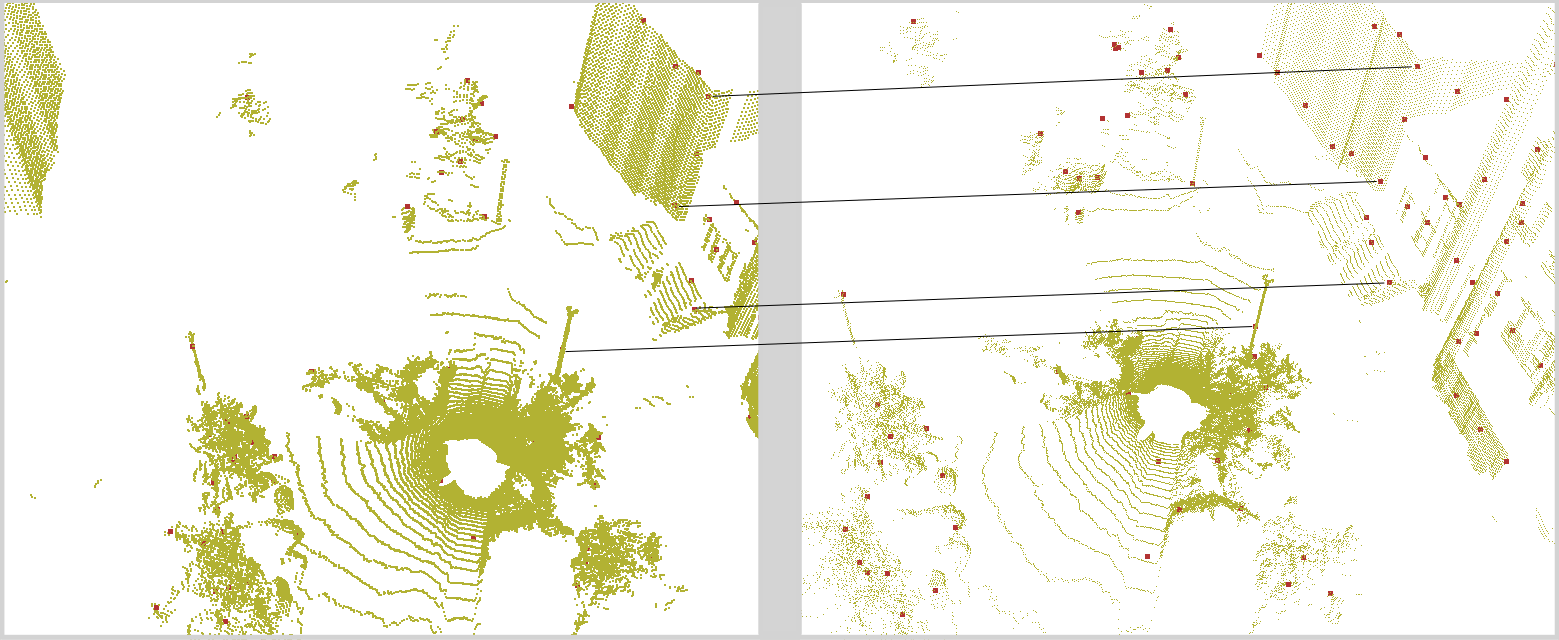
\includegraphics[width=0.995\linewidth]{img/chap_slam/features_line.png}\\
    \caption{Examples of NARF keypoints found for two different scans of the structured dataset. Black lines illustrate examples of valid correspondences found. These show stability under changes, such as viewpoint, noise and resolution.}
    \label{fig:chap_slam_features_correspondences}
\end{figure}


\subsection{Overview of the Algorithm}
\label{ssec:chap_slam_algo}

\todo{This section will give some more details about the NARF algorithm itself.}
~\citep[Section III, A]{Steder2011b}
\begin{itemize}
    \item Our system uses the estimated transformation to evaluate a candidate and in this way to more robustly reject false positives for place recognition
    \item Our approach transforms a given 3D range scan into a range image and uses a combination of a bag-of-words approach and a point-feature-based estimation of relative poses that are then individually scored
    \item Our algorithm described in this paper uses a novel feature type, an improved sensor model, includes a self- similarity analysis, and employs a bag-of-words approach as a preprocessing step to achieve a higher performance.
    \item In our former work on place recognition [16] we used point feature correspondences to find candidate transfor- mations between scans and calculated scores for those transformations.
    \item Rephrase this as intro : Given a database of 3D scans and a scan as input query, our algorithm returns a set of scans which are potential matches with the input. Additionally, it calculates for every returned scan a transformation and a score reflecting how certain the system is that the scans actually match
    \item Parameters: Descriptor size = 36, Max feature count = bow(2000) match(200), support size = bow(1/10 avg range) match(1/5 avg range)
    \item Basically what you want is to recopy III. A
    \item Note: using local descriptor allows to find the transformation between the two scans == localization
    \item Should I say that we used the rotation invariance param but it sucked
    \item BOW: they use the 3D scans, 2000 narf per scan, use k-means, choose closest word in euclidean, also euclidean for histogram.
    \item Each NARF encodes a full 3D transformation. Therefore, the knowledge about a single feature correspondence be- tween two scans enables us to retrieve all six degrees of freedom of the relative transformation between them (i.e., by calculating the difference between the two poses)
    \item To obtain the candidate transformations for each scan pair, we order the feature pairs according to increasing descriptor distance (see Section III-B) and evaluate the transformations in this order. In other words, we calculate a score for each of these transformations (see Section III-E) (they stop after 2000)
    \item The result of the feature matching is a list of relative poses Tk = Tk1,...,Tkn for the candidate pair ?. Our goal now is to evaluate those candidate transformations and calculate a score (likelihood) for each ? reflecting the confidence of the transformation given a model of our sensor
    \item Let P be a set of validation points from the query scan z*. This set P could contain all points from z* but we will only use a representative subset of z* as described at the end of this section.
    \item Section E describe the scoring method\dots 
    \item They compute a score for each point, then use these to compute the total score\dots. I cannot describe that, refer section III E
    \item Briefly talk about the self similarity (used to prevent false positives in area where very few distinctive structure like corridor)
    \item 
    \item 
    \item 
\end{itemize}

